\chapter*{Interacción lípido-péptido en monocapas de Langmuir} \label{mono}

 En este capítulo utilizamos monocapas de Langmuir para evaluar la estabilidad interfacial de los segmentos \ac{tm}-\ac{ic} de los péptidos $\alpha$IIb  y $\beta$3.

%%%%%%%%%%%%%%%%%%%%% Tabla pequeña %%%%%%%%%%%%%%%%%%%%%%%%

\begin{wraptable}{r}{5.8cm}
\vspace{-1.2cm} %%%Posiciona a una altura en la hoja
    \caption{Características de residuos para cada péptido.}\label{wrap-tab:1}
    \label{tab:secuencia}
    \begin{tabular}{lcr}
     \toprule  % <-- Toprule here
      {Residuos} & {$\alpha$IIb\%} & {$\beta$3\%}\\
      \hline
        \textcolor{mygreen}{Hidrofóbicos}   & 55.56 & 49.37\\
        \textcolor{blue}{Ácidos}            & 16.67 & 10.13\\
        \textcolor{red}{Básicos}            & 9.26  & 13.92\\
        \textcolor{black}{Neutros}          & 18.52 & 26.58\\ % <-- added row here
      \bottomrule % <-- Bottomrule here
      \textcolor{black}{Carga neta}            & 4-  & 2+\\
      \bottomrule % <-- Bottomrule here
    \end{tabular}
    \vspace{-0.5cm} %%%espacio entre texto y botton table
    \end{wraptable} 
%%%%%%%%%%%%%%%%%%%%% Fin %%%%%%%%%%%%%%%%%%%%%%%%
Antes de adentrarnos los resultados en monocapas, debemos analizar la estructura primaria y la secundaria de cada péptido. En la Figura~\ref{fig:secuencia} se resalta por característica cada grupo de residuos en colores diferentes, estas se resumen en la Tabla ~\ref{tab:secuencia}, la secuencia va desde el N al C terminal. Entre "\textbf{[ ]}" se resaltan los residuos que son efectivamente \ac{tm} y al lado izquierdo un pequeño loop \ac{EC} con residuos preferentemente hidrofóbicos y al lado derecho el tail \ac{ic} con residuos ácidos y básicos mayoritariamente para ambos péptidos, ésto último podría sugerir que el dominio \ac{ic} preferiría interactuar con el agua más que el loop \ac{ec} en el caso de estar expuesta a una subfase acuosa.

%%%%%%%%%%%%%%%%%%%%% Matrix Secuencia %%%%%%%%%%%%%%%%%%%%%%%%
\begin{figure}[ht]
    \centering
$\begin{NiceMatrix}

\text{$\alpha$}\text{IIb} &   &   &    &    &   &   &    &    &    &  &  &  &  &  & \\
955\text{--}969 & \textcolor{mygreen}{\mathrm{G}} & \textcolor{mygreen}{\mathrm{A}}& \textcolor{mygreen}{\mathrm{M}}& \textcolor{mygreen}{\mathrm{G}}& \textcolor{black}{\mathrm{S}}& \textcolor{red}{\mathrm{E}}& \textcolor{red}{\mathrm{E}}& \textcolor{blue}{\mathrm{R}}& \textcolor{mygreen}{\mathrm{A}} & \textcolor{mygreen}{\mathrm{I}} & \textbf{\Large[} \textcolor{mygreen}{\mathrm{P}} & \textcolor{mygreen}{\mathrm{I}} & \textcolor{mygreen}{\mathrm{W}} & \textcolor{mygreen}{\mathrm{W}} & \textcolor{mygreen}{\mathrm{V}} \\
970\text{--}984 &  \textcolor{mygreen}{\mathrm{L}} & \textcolor{mygreen}{\mathrm{V}} & \textcolor{mygreen}{\mathrm{G}} & \textcolor{mygreen}{\mathrm{V}} & \textcolor{mygreen}{\mathrm{L}} & \textcolor{mygreen}{\mathrm{G}} & \textcolor{mygreen}{\mathrm{G}} & \textcolor{mygreen}{\mathrm{L}} & \textcolor{mygreen}{\mathrm{L}}  & \textcolor{mygreen}{\mathrm{L}} & \textcolor{mygreen}{\mathrm{L}} & \textcolor{black}{\mathrm{T}} & \textcolor{mygreen}{\mathrm{I}} & \textcolor{mygreen}{\mathrm{L}} & \textcolor{mygreen}{\mathrm{V}}\\
985\text{--}999 &  \textcolor{mygreen}{\mathrm{L}} & \textcolor{mygreen}{\mathrm{A}} & \textcolor{mygreen}{\mathrm{M}} & \textcolor{mygreen}{\mathrm{W}} & \textcolor{blue}{\mathrm{K}} & \textcolor{mygreen}{\mathrm{V}} & \textcolor{mygreen}{\mathrm{G}} & \textcolor{mygreen}{\mathrm{F}}\textbf{\Large]} & \textcolor{mygreen}{\mathrm{F}} & \textcolor{blue}{\mathrm{K}} & \textcolor{blue}{\mathrm{R}} & \textcolor{black}{\mathrm{N}} & \textcolor{blue}{\mathrm{R}} & \textcolor{mygreen}{\mathrm{P}} & \textcolor{mygreen}{\mathrm{P}} &\\
1000\text{--}1008  & \textcolor{mygreen}{\mathrm{L}}& \textcolor{red}{\mathrm{E}} & \textcolor{red}{\mathrm{E}} & \textcolor{red}{\mathrm{D}} & \textcolor{red}{\mathrm{D}} & \textcolor{red}{\mathrm{E}} & \textcolor{red}{\mathrm{E}} & \textcolor{mygreen}{\mathrm{G}} & \textcolor{red}{\mathrm{E}} \\

\text{$\beta$}3 \\
684\text{--}698 &    \textcolor{mygreen}{\mathrm{G}} & \textcolor{mygreen}{\mathrm{A}} & \textcolor{mygreen}{\mathrm{M}} & \textcolor{mygreen}{\mathrm{G}} & \textcolor{black}{\mathrm{S}} & \textcolor{blue}{\mathrm{K}} & \textcolor{mygreen}{\mathrm{G}} & \textcolor{mygreen}{\mathrm{P}} & \textcolor{red}{\mathrm{D}} & \textcolor{mygreen}{\mathrm{I}} & \textbf{\Large[}\textcolor{mygreen}{\mathrm{L}} & \textcolor{mygreen}{\mathrm{V}} & \textcolor{mygreen}{\mathrm{V}} & \textcolor{mygreen}{\mathrm{L}} & \textcolor{mygreen}{\mathrm{L}}\\
699\text{--}713  &  \textcolor{black}{\mathrm{S}} & \textcolor{mygreen}{\mathrm{V}} &  \textcolor{mygreen}{\mathrm{M}} & \textcolor{mygreen}{\mathrm{G}} & \textcolor{mygreen}{\mathrm{A}} & \textcolor{mygreen}{\mathrm{I}} & \textcolor{mygreen}{\mathrm{L}} & \textcolor{mygreen}{\mathrm{L}} & \textcolor{mygreen}{\mathrm{I}} & \textcolor{mygreen}{\mathrm{G}} &  \textcolor{mygreen}{\mathrm{L}} & \textcolor{mygreen}{\mathrm{A}} & \textcolor{mygreen}{\mathrm{A}} & \textcolor{mygreen}{\mathrm{L}} & \textcolor{mygreen}{\mathrm{L}}\\
714\text{--}728 & \textcolor{mygreen}{\mathrm{I}} & \textcolor{mygreen}{\mathrm{W}} & \textcolor{blue}{\mathrm{K}} & \textcolor{mygreen}{\mathrm{L}} & \textcolor{mygreen}{\mathrm{L}} & \textcolor{mygreen}{\mathrm{I}} & \textcolor{black}{\mathrm{T}} & \textcolor{mygreen}{\mathrm{I}}\textbf{\Large]} & \textcolor{mygreen}{\mathrm{H}} & \textcolor{red}{\mathrm{D}} & \textcolor{blue}{\mathrm{R}} & \textcolor{blue}{\mathrm{K}} & \textcolor{red}{\mathrm{E}} & \textcolor{mygreen}{\mathrm{F}} & \textcolor{mygreen}{\mathrm{A}} & \\
729\text{--}743 & \textcolor{blue}{\mathrm{K}} & \textcolor{mygreen}{\mathrm{F}} & \textcolor{red}{\mathrm{E}} & \textcolor{red}{\mathrm{E}} & \textcolor{red}{\mathrm{E}} & \textcolor{blue}{\mathrm{R}} & \textcolor{mygreen}{\mathrm{A}} & \textcolor{blue}{\mathrm{R}} & \textcolor{mygreen}{\mathrm{A}} & \textcolor{blue}{\mathrm{K}} & \textcolor{mygreen}{\mathrm{W}} & \textcolor{red}{\mathrm{D}} & \textcolor{black}{\mathrm{T}} & \textcolor{mygreen}{\mathrm{A}} & \textcolor{black}{\mathrm{N}} &  \\
744\text{--}758 & \textcolor{black}{\mathrm{N}} & \textcolor{mygreen}{\mathrm{P}} & \textcolor{mygreen}{\mathrm{L}} & \textcolor{black}{\mathrm{Y}} & \textcolor{blue}{\mathrm{K}} & \textcolor{red}{\mathrm{E}} & \textcolor{mygreen}{\mathrm{A}} & \textcolor{black}{\mathrm{T}} & \textcolor{black}{\mathrm{S}} & \textcolor{black}{\mathrm{T}} & \textcolor{mygreen}{\mathrm{F}} & \textcolor{black}{\mathrm{T}} & \textcolor{black}{\mathrm{N}} & \textcolor{mygreen}{\mathrm{I}} & \textcolor{black}{\mathrm{T}}\\
759\text{--}762 & \textcolor{black}{\mathrm{Y}} & \textcolor{blue}{\mathrm{R}} & \textcolor{mygreen}{\mathrm{G}} & \textcolor{black}{\mathrm{T}} \\
\end{NiceMatrix}$ \\
   
    \caption{Características de cada amino ácido para las secuencias de $\alpha$IIb y $\beta$3. Los colores de cada letra corresponden a las propiedades por residuo, \textcolor{mygreen}{verde: hidrofóbicos (G F I L M V W A P)}, \textcolor{blue}{azul: básicos (R K H (+))}, \textcolor{red}{rojo: ácidos (D E (-))}, \textcolor{black}{negro: otros (S T N Y)}. Datos extraídos de \url{https://www.peptide2.com/N_peptide_hydrophobicity_hydrophilicity.php}.
    }
    \label{fig:secuencia}
\end{figure}
%%%%%%%%%%%%%%%%%%%%% Fin %%%%%%%%%%%%%%%%%%%%%%%%
Además, surge pregunta la ¿cómo se orientan los péptidos en la interfase aire-agua?. En las proteínas nativas, ambos péptidos tienen estructura $\alpha$ hélice; si consideramos a un péptido transmembrana como un cilindro (Figura ~\ref{fig:orientTM}-\textbf{b}), podemos inferir acerca de su orientación a partir de las medidas de área molecular en capas monomoleculares. Un área molecular experimental similar al área del cilindro indicaría un arreglo de péptidos orientados perpendicularmente a la interfase y altamente compactados con se representa en la Figura ~\ref{fig:orientTM}-\textbf{a}-\textit{ii}. Valores mayores de área molecular corresponderían a otras orientaciones no perpendiculares.

%%%%%%%%%%%%%%%%%%%%% Fig {Modelo de posible orientación %%%%%%%%%%%%%%%%%%%%%%%%
%\begin{figure}[h] % supposedly places it here ...
%    \centering
%	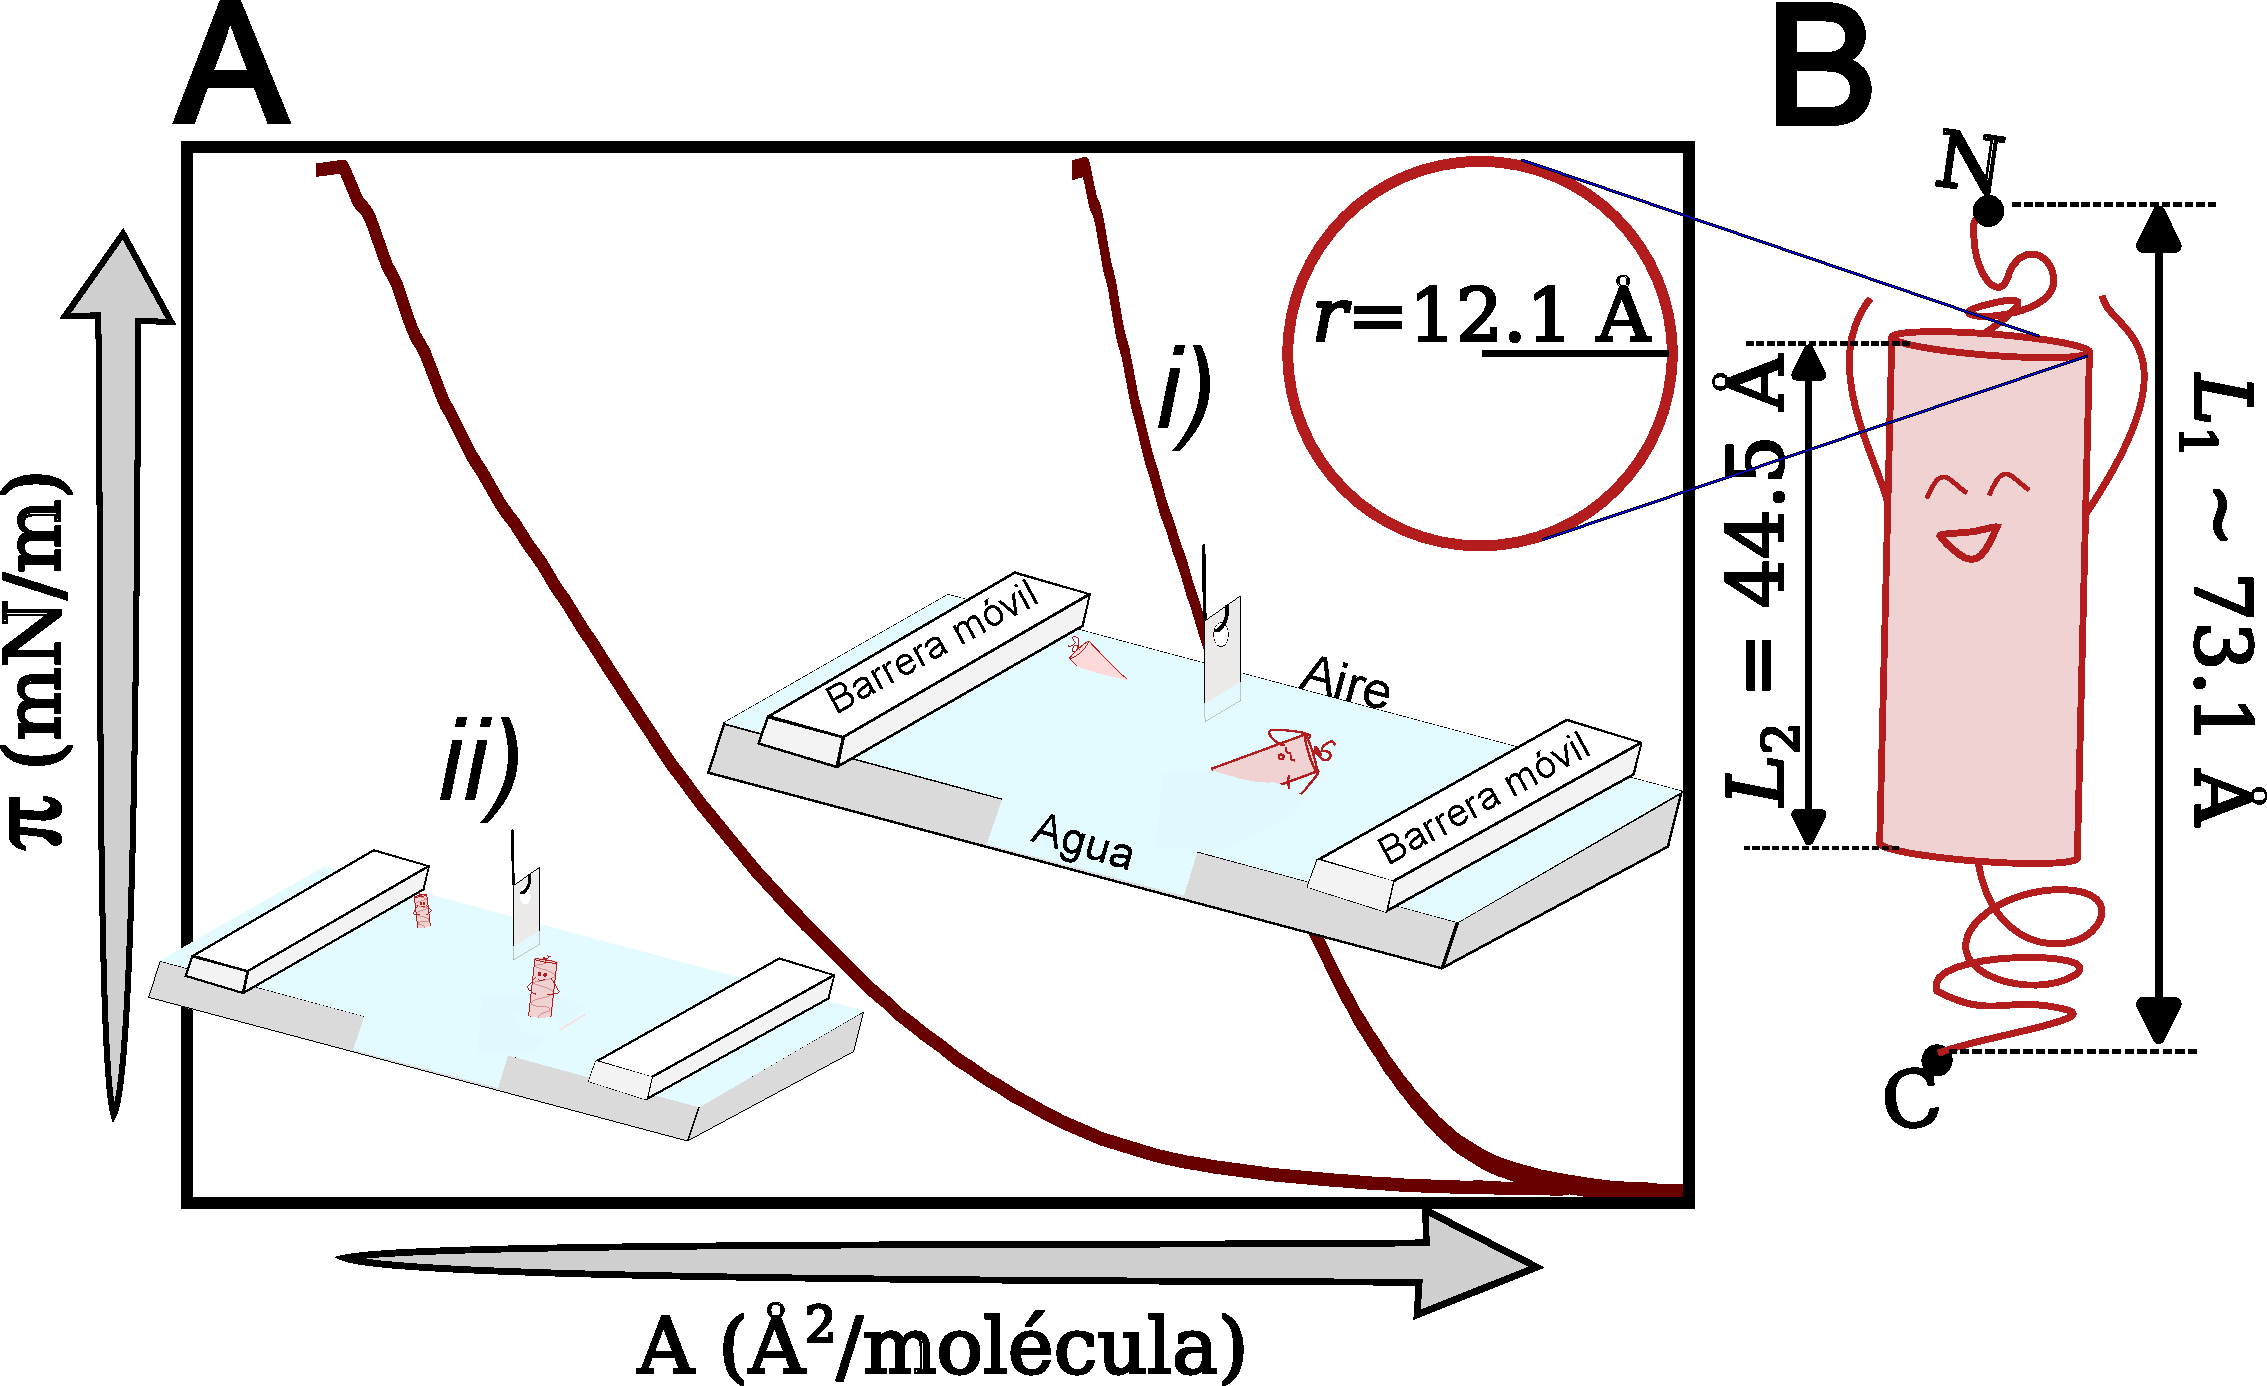
\includegraphics[width=0.79\linewidth]{fig/01_expe/orienta_pept2.pdf}
%	\caption{Modelo de posible orientación de $\alpha$-hélice en el plano de una monocapa.}
%        \index{orientacion}
%    \label{fig:orientTM}
%\end{figure}
%%%%%%%%%%%%%%%%%%%%% Fin %%%%%%%%%%%%%%%%%%%%%%%%

%\begin{figure}[h] % supposedly places it here ...
%    \centering
%	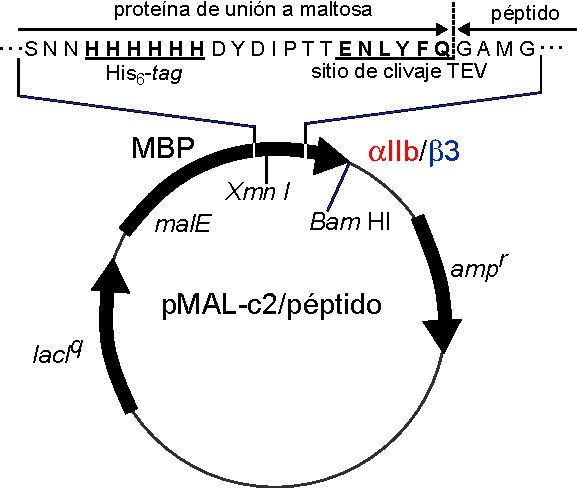
\includegraphics[width=0.79\linewidth]{fig/01_expe/pmal_c2.pdf}
%	\caption{Esquema plásmido pMAL-c2 - $\alpha$IIb/$\beta$3. Figura adaptada de Vector Database por \href{https://www.addgene.org/}{addgene.org} (2023). Extraído de \url{https://www.addgene.org/vector-database/3506/}.}
%        \index{plasmido}
%    \label{fig:plasmido}
%\end{figure}


\section{Influencia de segmentos \ac{tm}-\ac{ic}  $\alpha$IIb  y $\beta$3 en monocapas de Langmuir}

Las isotermas $\pi$--A pueden emplearse para obtener información acerca de la estructura, área, compresibilidad, histéresis, transición de fase, cambios conformacionales e interacciones entre monocapas de lípido y proteína/péptido. Se realizaron experimentos de monocapas de Langmuir con la finalidad de deducir cuál era la orientación de cada uno de los segmentos \ac{TM} de integrinas en superficie la de la interfase aire-agua y el efecto inducido por la presencia de los péptidos en las monocapas de POPC, DPPC y POPC:POPG 70:30 (PCPG).

\subsection{Monocapas péptidos puros}

En la Figura~\ref{fig:alfa_pi_A} \textbf{a, f}, se muestra la isoterma para los péptidos puros donde se toma como presión de referencia 30 mN/m, al ser considerada la presión de referencia en las membranas biológicas \hl{[ref xx-yy]}. El área molecular a esa presión fue de $482 \pm 52$ y $593 \pm 20$ Å\textsuperscript{2} para $\alpha$IIb y $\beta$3, respectivamente. Los ciclos de compresión--expansión (Figura~\ref{fig:compre_expan}) sugieren que ambos péptidos forman monocapas estables. Como se mencionó anteriormente acerca de la posible orientación de los péptidos en el plano de la monocapa, consideremos el largo (L$_1$) del péptido (Figura~\ref{fig:orientTM}-\textbf{b}) como el radio del cilindro, para lo cual daría un área molecular promedio de $16471$ Å\textsuperscript{2} para $\alpha$IIb y $35968$ Å\textsuperscript{2} para $\beta$3. Por literatura se sabe \hl{[ref bb-cc]} que un péptido con estructura $\alpha$-hélice.

presenta un radio entre 5-15 Å\textsuperscript{2} el cual varia según la longitud de la cadena peptídica, por lo tanto, el área menor a ocupar ronda cerca de los 78 Å\textsuperscript{2}molécula.  Las áreas observadas experimentalmente se encuentran muy alejadas de la condición donde los péptidos estarían paralelos a plano de la monocapa, al contrario parecen indicar que ambos péptidos tienden a orientarse perpendicularmente. Se observa un incremento del potencial de superficie ($\Delta$V)  que va desde los 150-200 mV hasta 300 mV para ambos péptidos, al llegar a los $\approx$ 350 {Å\textsuperscript{2} la señal del potencial presentó un cambio de tendencia donde deja de incrementar y quedó casi constante, esto podría ser porque esa área las moléculas se encuentran lo suficientemente compactas.


\subsection{Monocapas mezclas lípido-péptido}

Las isotermas de compresión del péptido $\alpha$IIb puro y mezcla lípido-péptido desde 0.0 a 7.0\% mol de $\alpha$IIb  se muestra en la Figura ~\ref{fig:alfa_pi_A} \textbf{a-d}, en todos los experimentos se realizaron 3 ciclos de compresión-expansión para evaluar la estabilidad del film lípido-péptido. Para la mezcla \ac{POPC}:$\alpha$IIb se observa que en todos los casos se produjo un corrimiento a áreas mayores cuando hay presencia de péptido y este aumenta con el incremento de la concentración. Para la mezcla con \ac{dppc} se observa un corrimiento a áreas mayores más marcado comparado al que se produjo con \ac{POPC}, y de forma similar, ese desplazamiento parece aumento con la concentración; y cuando el péptido esta en presencia de la mezcla binaria PCPG (POPC:POPG 70:30 mol a mol) este comportamiento ya no sigue dicha tendencia.
El potencial de superficie (- -, $\Delta$V) para las tres mezclas lípido-péptido el incremento es mínimo comparado a la señal del $\Delta$V de los lípidos puros (\textbf{\Large{-\large{\faTimes}-}}), pareciera que las concentraciones evaluadas no se produce un cambio notable en el $\Delta$V.

\definecolor{falured}{rgb}{0.5, 0.09, 0.09} %%2.0%
\definecolor{emerald}{rgb}{0.31, 0.78, 0.47} %%%3.5%
\definecolor{goldenpoppy}{rgb}{0.99, 0.76, 0.0} %%5.0
\definecolor{deepmagenta}{rgb}{0.8, 0.0, 0.8}  %%7.0%

Por otra lado, en la Figura ~\ref{fig:alfa_pi_A} \textbf{e-h} se observan las isotermas en presencia de $\beta$3. Para las mezclas lípido-péptido en POPC y PCPG se observa que a concentraciones de 2.0\% (\textcolor{emerald}{\rotatebox{0}{\faStar}})  y 3.5\% (\textcolor{falured}{\rotatebox{90}{\faPlay}}) no se ve un corrimiento marcado como sucedió en presencia de $\alpha$IIb, incluso se ve que en todas las concentraciones de péptido la isoterma de la mezcla o no se diferencia del lípido puro o incluso se corre a áreas menores (Figura ~\ref{fig:alfa_pi_A} \textbf{h}). Para \ac{dppc} el comportamiento fue muy similar al observado en presencia de $\alpha$IIb. Respecto a los $\Delta$V, de nuevo para \ac{POPC} y \ac{dppc} hay una leve tendencia a aumentar con el incremento de la concentración del péptido, sin embargo, para PCPG para todas las mezclas, excepto a 2.0\%, la señal del potencial disminuyó respecto a la mezcla de lípido sin péptido. A 2.0$\%$ de $\beta$3 el $\Delta$V presentó un comportamiento muy diferentes a las otras concentraciones donde al inicio de la compresión la señal subió cerca de 390 mV y luego permaneció casi constante hasta los 75 Å\textsuperscript{2}y luego cayó a valores cercanos de 325 mV, similares a las otras concentraciones de péptido.

Ahora, comparando un poco más en detalle el efecto de los dos péptidos,  en las monocapas de \ac{popc}, a 5.0\% (\textcolor{goldenpoppy}{\faCircle}) de $\alpha$IIb se desplaza a área menores comparado las concentraciones más bajas que iba aumentando pero luego a 7.0\% (\textcolor{deepmagenta}{\faCircle}) se recupera dicha tendencia, mientras que en presencia de $\beta$3 sucede el mismo efecto pero a 2.0\% y luego se produce el corrimiento a áreas mayores. En presencia de \ac{dppc} el corrimiento hacia áreas mayores al incrementar la concentración de péptido se cumple para ambos péptidos, sin embargo, en presencia de $\beta$3 esa tendencia se sigue hasta 5.0$\%$ porque luego a 7.0\% baja a corrimientos similares al 2.0\% de $\beta$3.

Dado que de los gráficos anteriores no se puede realizar conclusiones generales, se procedió a realizar un análisis del área molecular promedio Vs el porcentaje de péptido a diferentes presiones con la finalidad de encontrar alguna tendencia más evidente para cada sistema estudiado (ver sección ~\ref{AvsMol}).
%%%%%%%%%%%%%%%%%%%%%Fig. Isotermas de compresión %%%%%%%%%%%%%%%%%%%%%


%\begin{figure}[H]
%    \centering
%    \begin{subfigure}[t]{0.45\textwidth}
%        \centering
%        \subcaption{}
%        \includegraphics[width=1\linewidth, height=0.30\textheight, keepaspectratio]{fig/01_expe/mono/alfa_beta_dV.eps} 
%    \end{subfigure}
%    \begin{subfigure}[t]{0.45\textwidth}
%        \centering
%        \subcaption{}
%        \includegraphics[width=1\linewidth, height=0.30\textheight, keepaspectratio]{fig/01_expe/mono/alfa_popc_avg_V.eps}     
%    \end{subfigure}
    
%    \begin{subfigure}[t]{0.45\textwidth}
%        \centering
%        \subcaption{}
%        \includegraphics[width=1\linewidth, height=0.30\textheight, keepaspectratio]{02_figuras/01_Fig_experime/mono/alfa_dppc_avg_V.eps}  
%    \end{subfigure}
%    \begin{subfigure}[t]{0.45\textwidth}
%        \centering
%        \subcaption{}
%        \includegraphics[width=1\linewidth, height=0.30\textheight, keepaspectratio]{02_figuras/01_Fig_experime/mono/alfa_pcpg_avg_V.eps}  
%    \end{subfigure}
%
%    \bottomrule % <-- Bottomrule here
%
%    \begin{subfigure}[t]{0.45\textwidth}
%        \centering
%        \subcaption{}
%        \includegraphics[width=1\linewidth, height=0.30\textheight, keepaspectratio]{02_figuras/01_Fig_experime/mono/beta_dV.eps} 
%    \end{subfigure}
%    \begin{subfigure}[t]{0.45\textwidth}
%        \centering
%        \subcaption{}
%        \includegraphics[width=1\linewidth, height=0.30\textheight, keepaspectratio]{02_figuras/01_Fig_experime/mono/beta_popc_avg_V.eps}     
%    \end{subfigure}
%    
%    \begin{subfigure}[t]{0.45\textwidth}
%        \centering
%        \subcaption{}
%        \includegraphics[width=1\linewidth, height=0.30\textheight, keepaspectratio]{02_figuras/01_Fig_experime/mono/beta_dppc_avg_V.eps}  
%    \end{subfigure}
%    \begin{subfigure}[t]{0.45\textwidth}
%        \centering
%        \subcaption{}
%        \includegraphics[width=1\linewidth, height=0.30\textheight, keepaspectratio]{02_figuras/01_Fig_experime/mono/beta_pcpg_avg_V.eps}  
%    \end{subfigure}


%\caption{Isotermas de compresión, presión superficial -- área molecular promedio ($\pi$--A) en la interfase aire-agua para \textbf{a-d)} péptido $\alpha$IIb y \textbf{e-f)} péptido $\beta$3 y, mezclas lípido-péptido \textbf{b-c-d)} POPC, DPPC y PCPG, respectivamente. Las líneas suspendidas (- -) corresponden al potencial de superficie ($\Delta$V).
%        \index{alfa_pi_A}}
%    \label{fig:alfa_pi_A}
%\end{figure}
%%%%%%%%%%%%%%%%%%%%%%%FIN%%%%%%%%%%%%%%%%%%%%%%%%%%%%%%%%%%%%%%%%%

%
%
%%%%%%%%%% Àrea Vs %mol
\section{Área molecular Vs porcentaje de péptido}{\label{AvsMol}}

A partir de los datos de la Figura ~\ref{fig:alfa_pi_A} se extrajo información acerca del área molecular promedio Vs el porcentaje en mol de cada péptido y se tomaron diferentes presiones de referencia (Figura ~\ref{fig:AreaVsMoles}), éstas se compararon  respecto a valores ideales a determinada presión con la finalidad analizar la interacción lípido-péptido, el cálculos de la curva ideal fue calculada según la ecuación:
%
%\begin{equation}
%    \label{Aideal}
%    A_{ideal} = \left[X_{\text{L}}A_{\text{L}} + X_{\text{P}}A_{\text{P}}\right]_\pi
%\end{equation}

Donde $A_{L}$ y $A_{P}$ son las áreas moleculares promedio de los lípidos y los péptidos, respectivamente, $X_{L}$ y $X_{P}$ son las fracciones molares de lípido y péptido a una determinada presión.
Para monocapas de \ac{popc}, en todas las presiones evaluadas los resultados sugieren que ambos péptidos parecen interaccionar atractivamente con lípidos, es decir, en presencia de péptido los lípidos tienden a compactarse y éste comportamiento es más evidente a presiones bajas como 2 y 5 mN/m. Para el caso de $\alpha$IIb se que a 5\% mol se compacta más que en las otras concentraciones, tal como se observó en la Figura ~\ref{fig:alfa_pi_A} \textbf{b}. En el caso de \ac{dppc} sucedió lo contrario, las áreas experimentales en ambos péptidos fueron mayores a las áreas ideales, lo cual sugiere que la interacción lípido-péptido no se favorece o es de carácter repulsivo y por lo tanto, la monocapa se expande. Los dos péptidos inducen el mismo efecto hasta una concentración de 5.0\% y a 7.0\% tiende a compactarse un poco el sistema, sin embargo, se observa que el péptido $\beta$3 es quien induce un mayor corrimiento a área mayores, respecto a lo observado con $\alpha$IIb. Una posible explicación para esta diferencia puede resultar en la diferencia de tamaño de los péptidos donde $\beta$3 tiene una \hl{cola} \ac{IC} más larga que $\alpha$IIb y ésta puede moverse con mayor libertar y por ende, podría estar ocupando un mayor área, sin embargo al aumentar la concentración de péptido, las moléculas tendrían menor libertad de movimiento y por lo tanto, tiende a compactarse como sucede a 7\%. De forma similar como sucedió en las monocapas de \ac{popc}, a presiones bajas el efecto repulsivo es más evidente que presiones altas como 30 mN/m.
Por último, en las monocapas de PCPG (Figura ~\ref{fig:AreaVsMoles} \textbf{e-f}), la presencia de $\alpha$IIb a bajas concentraciones (2.0\% y 3.5\%) tiende a comportarse como una mezcla ideal, luego a 5.0\% y 7.0\% la mezcla lípido-péptido tiende a compactarse, deduciendo que se favorece la interacción lípido-péptido. A 5.0\% mol de péptido se observó la mayor compactación, tal como se vio la Figura ~\ref{fig:alfa_pi_A} \textbf{d}. En cuando al efecto inducido por $\beta$3, se observó un corrimiento a áreas menores en todas las concentraciones, siendo más pronunciada a 3.5\% y 5.0\% y ese corrimiento es más grande que el que induce el péptido $\alpha$IIb. La diferencia del efecto inducido en la monocopa por cada péptido, podría atribuirse a la carga neta, $\beta$3 tiene carga 2+ la cual posiblemente podría verse atraída por la carga negativa del PG, mientras que $\alpha$IIb su carga es de 4- la cual podría estar repeliendo las carga del PG en la mezcla PCPG.

%%%%%%%%%%%%%%%%%%%%%% Fig A Vs %mol %%%%%%%%%%%%%%%%%%%%%%%%
%\begin{figure}[H]
%    \centering
%    
%    \begin{subfigure}[t]{0.49\textwidth}
%        \centering
%        \subcaption{}
%        \includegraphics[width=1.0\linewidth, height=0.30\textheight, keepaspectratio]
%        {02_figuras/01_Fig_experime/mono/alfa_popc_2_30pi.eps}  
%    \end{subfigure}
%    \begin{subfigure}[t]{0.49\textwidth}
%        \centering
%        \subcaption{}
%        \includegraphics[width=1.0\linewidth, height=0.30\textheight, keepaspectratio]
%        {02_figuras/01_Fig_experime/mono/beta_popc_2_30pi.eps} 
%    \end{subfigure}
%    
%    \begin{subfigure}[t]{0.49\textwidth}
%        \centering
%        \subcaption{}
%        \includegraphics[width=1.0\linewidth, height=0.30\textheight, keepaspectratio]
%        {02_figuras/01_Fig_experime/mono/alfa_dppc_2_30pi.eps}  
%    \end{subfigure}
%    \begin{subfigure}[t]{0.49\textwidth}
%        \centering
%        \subcaption{}
%        \includegraphics[width=1.0\linewidth, height=0.30\textheight, keepaspectratio]
%        {02_figuras/01_Fig_experime/mono/beta_dppc_2_30pi.eps} 
%    \end{subfigure}
%
%    \begin{subfigure}[t]{0.49\textwidth}
%        \centering
%        \subcaption{}
%        \includegraphics[width=1.0\linewidth, height=0.30\textheight, keepaspectratio]
%        {02_figuras/01_Fig_experime/mono/alfa_pcpg_2_30pi.eps}  
%    \end{subfigure}
%    \begin{subfigure}[t]{0.49\textwidth}
%        \centering
%        \subcaption{}
%        \includegraphics[width=1.0\linewidth, height=0.30\textheight, keepaspectratio]
%        {02_figuras/01_Fig_experime/mono/beta_pcpg_2_30pi.eps}
%    \end{subfigure}
%
%    \caption{Área molecular promedio Vs fracción molar de péptido a diferentes presiones. \textbf{a-b)} POPC, \textbf{c-d)} DPPC y \textbf{e-f)} PCPG. Las líneas \textbf{- -} corresponden a la curva ideal y las líneas \textbf{\Large{--}} a los resultados experimentales.}
%    \index{Fig_AreaVsMoles}
%    \label{fig:AreaVsMoles}
%\end{figure}
%%%%%%%%%%%%%%%%%%%%%% Fin %%%%%%%%%%%%%%%%%%%%%%%%
%d
%
%%%%Paper Properties of the Langmuir and Langmuir–Blodgett monolayers
%%%%of cholesterol‑cyclosporine A on water and polymer support
%%%%https://doi.org/10.1007/s10450-019-00117-2
%
%\subsection{Módulo de compresibilidad}{}
%%%%%%% P. Módulo de compresibilidad

Se calcularon los módulos de compresibilidad (C$_s^{\text{--}1}$) para cada monocapa empleando la ecuación ~\ref{Cs} y se graficaron en función de la presión superficial (Figura ~\ref{fig:CsPi}) con la finalidad de obtener información relacionada con la elasticidad en el plano de la superficie [\hl{ref: Davies and Rideal (1963)}]. Los autores Davies and Rideal encontraron para los estados líquido expandido (LE) y líquido condensado (LC) los valores de C$_s^{\text{--}1}$ estan en los rangos de 12.5-50 mN/m y 100-250 mN/m. Mientras que los para el estado sólido (S), el C$_s^{\text{--}1}$  varía entre 1000-2000 mN/m.

\begin{equation} 
    \label{Cs}
    C_s^{\text{--}1} = \frac{1}{A}\left(\frac{dA}{d\pi} \right)  
\end{equation}
%
%
%
%%%%%%%%%% Figura Módulo de compresibilidad %%%%%%%%%%%%
%\begin{figure}[H]
%
%    \centering
%    \begin{subfigure}[t]{0.49\textwidth} %%%%ajustar el 0.xx para que fit a la página
%        \centering
%        \subcaption{}
%        \includegraphics[width=1.0\linewidth, height=0.30\textheight, keepaspectratio]
%        {02_figuras/01_Fig_experime/mono/alfa_popc_Cs.eps}  
%    \end{subfigure}
%    \begin{subfigure}[t]{0.49\textwidth}
%        \centering
%        \subcaption{}
%        \includegraphics[width=1.0\linewidth, height=0.30\textheight, keepaspectratio]
%        {02_figuras/01_Fig_experime/mono/beta_popc_Cs.eps} 
%    \end{subfigure}
%    
%    \begin{subfigure}[t]{0.49\textwidth}
%        \centering
%        \subcaption{}
%        \includegraphics[width=1.0\linewidth, height=0.30\textheight, keepaspectratio]
%        {02_figuras/01_Fig_experime/mono/alfa_dppc_Cs.eps}  
%
%    \end{subfigure}
%    \begin{subfigure}[t]{0.49\textwidth}
%        \centering
%        \subcaption{}
%        \includegraphics[width=1.0\linewidth, height=0.30\textheight, keepaspectratio]
%        {02_figuras/01_Fig_experime/mono/beta_dppc_Cs.eps}  
%    \end{subfigure}
%
%
%    \begin{subfigure}[t]{0.49\textwidth}
%        \centering
%        \subcaption{}
%        \includegraphics[width=1.0\linewidth, height=0.30\textheight, keepaspectratio]
%        {02_figuras/01_Fig_experime/mono/alfa_pcpg_Cs.eps}  
%    \end{subfigure}
%    \begin{subfigure}[t]{0.49\textwidth}
%        \centering
%        \subcaption{}
%        \includegraphics[width=1.0\linewidth, height=0.30\textheight, keepaspectratio]
%        {02_figuras/01_Fig_experime/mono/beta_pcpg_Cs.eps}
%    \end{subfigure}
%
%\caption{Módulo de compresibilidad Vs presión superficial en la interfase aire-agua para \textbf{a-b)} POPC, \textbf{c-d)} DPPC y \textbf{e-f)} PCPG, en presencia y ausencia de $\alpha$IIb o $\beta$3.}
%        \index{CsPi}
%    \label{fig:CsPi}
%\end{figure}
%
%%%%%%%%%%%%%%%%%%%%%% Fin %%%%%%%%%%%%%%%%%%%%%%%%

Tanto para POPC, DPPC y PCPG, se observa que $\alpha$IIb presenta un C$_s^{-1}$ que oscila cerca de los 35 mN/m cuando alcanza las presiones de 8-40 mN/m, para $\beta$3 C$_s^{-1}$ oscila cerca de los 30 mN/m. En este rango de presiones alcanzado se podría atribuir a características del estado LE; y como era de esperar para el POPC puro presentan un C$_s^{-1}$ de características de LE en todo el rango de $\pi$ (Figura ~\ref{fig:CsPi} \textbf{a-b}). Para las mezclas lípido-péptido, a medida que se incrementa la concentración de péptido, el C$_s^{-1}$ aumenta. Se observa que cuando el \% molar de péptido es 5-7, se alcanzan valores de C$_s^{-1}$ mayores a 50 mN/m, lo cual podría tratarse de un estado intermedio entre LE y LC.

Para DPPC Figura ~\ref{fig:CsPi} \textbf{c-d}, en el lípido puro se observan dos estados, principalmente, el primero alcanza un valor de C$_s^{\text{--}1}$  ~25 mN/m que alcanza rápidamente entre valore de $\pi$ de 0-12.5 mN/m, éste primer estado correspondería a la transición entre LE a LC. Posteriormente se produce un aumento pronunciado del C$_s^{-1}$ con el amento de la $\pi$ hasta alcanzar valores de C$_s^{\text{--}1}$  110 mN/m, lo cual se trata de una estado de LC. Cuando se adiciona péptido ya sea $\alpha$IIb o $\beta$3, la tendencia a aumentar el C$_s^{\text{--}1}$  se corresponde con el incremento de la concentración de péptido, sin embargo los valores de C$_s^{\text{--}1}$ alcanzados son más grandes comparados a los del lípido puro, incluso en el primer rango de presiones de 0-12.5 mN/m donde el C$_s^{\text{--}1}$ alcanza valores de 62 mN/m, después se alcanza valores máximos C$_s^{\text{--}1}$ 60 mN/m.

Por otra parte, cuando hay presencia de POPG (Figura ~\ref{fig:CsPi} \textbf{e-f}), para los dos péptidos los valores de C$_s^{\text{--}1}$ dismunuyen, comparados a los C$_s^{\text{--}1}$ tanto de la mezcla de lípido PCPG como los péptidos puros y los valores de C$_s^{\text{--}1}$  tienden a aumentar con el incremento del \%molar de péptido pero en todos los casos el C$_s^{\text{--}1}$ está por debajo de los 30 mN/m, lo cual indica que se trata de un estado LE en todo el rango de presiones.


En general para POPC se observa una tendencia a aumentar el C$_s^{\text{--}1}$ en presencia de $\alpha$IIb  o $\beta$3, los valores obtenidos para la concentración más alta de péptido (7.0\% mol, \textcolor{deepmagenta}{\faSquare}). El perfil de las curvas nos indica que al aumentar la concentración de péptido, aumenta la compresibilidad, lo cual se puede interpretar como que se forma un films más compacto (valores mayores de C$_s^{\text{--}1}$ respecto  a los lípidos puros. De forma similar se observó que los valores de C$_s^{\text{--}1}$ en monocapas de DPPC tienden a aumentar (excepto a 7.0\%) al incrementar el porcentaje de péptido. Además, en todas las concentraciones de de cada péptido se observa evidentemente al menos dos transiciones de fase, la primera entre 0-12.5 mN/m y pareciera observarse otra entre 14-23 mN/m ($\pi$), la primera correspondería a la fase líquido condensado (\hl{LC}), la segunda a (\hl{LE}) y por último entre 23-44 mN/m podría atribuirse al estado S (condensado).

La presencia del POPG en la monocapa de PCPG, indujo el efecto opuesto a los dos casos anteriores, los valores de C$_s^{\text{--}1}$ toma valores menores a los de la mezcla de lípidos y péptidos puros en todo el rango de presiones, lo cual indica que se forma un film con características de LE.

%%%%%%%%% Ciclos compresion-Expansión%%%%%%
\section{Histéresis}

Se estudió la histéresis del sistema en monocapas, realizando ciclos de compresión - expansión, con la finalidad de determinar la estabilidad de los péptidos en la monocapa. Si al realizar diferentes los ciclos los péptidos se desorbe de la monocapa, se observaría un corrimiento de las áreas en los diferentes ciclos, éste proceso se conoce como histéresis  (\hl{Ref}).  Los resultados se muestran en la Figura ~\ref{fig:compre_expan}, las monocapas de los péptidos puros como las mezclas péptido/lípido en las diferentes composiciones, se observan que son estables, es decir, al realizar los diferentes ciclos de compresión-expansión al parecer no se observa migración de muestra hacia la subfase, concluyendo así que en todos los casos se forma un film estable.\\
\hl{Me faltan incluir al grafico los de PCPG pero ya la grafica quedaba muy saturada, quizas si conviene incluirlas debo organizarlas de forma diferente}

%%%%%%%%Hoja horizontal %%%%%%%%%%%%%%%%%%%%%%%%
\begin{landscape}
%\thispagestyle{mylandscape} %Call our predefined page type

\begin{figure}[] % supposedly places it here ...
    \centering
    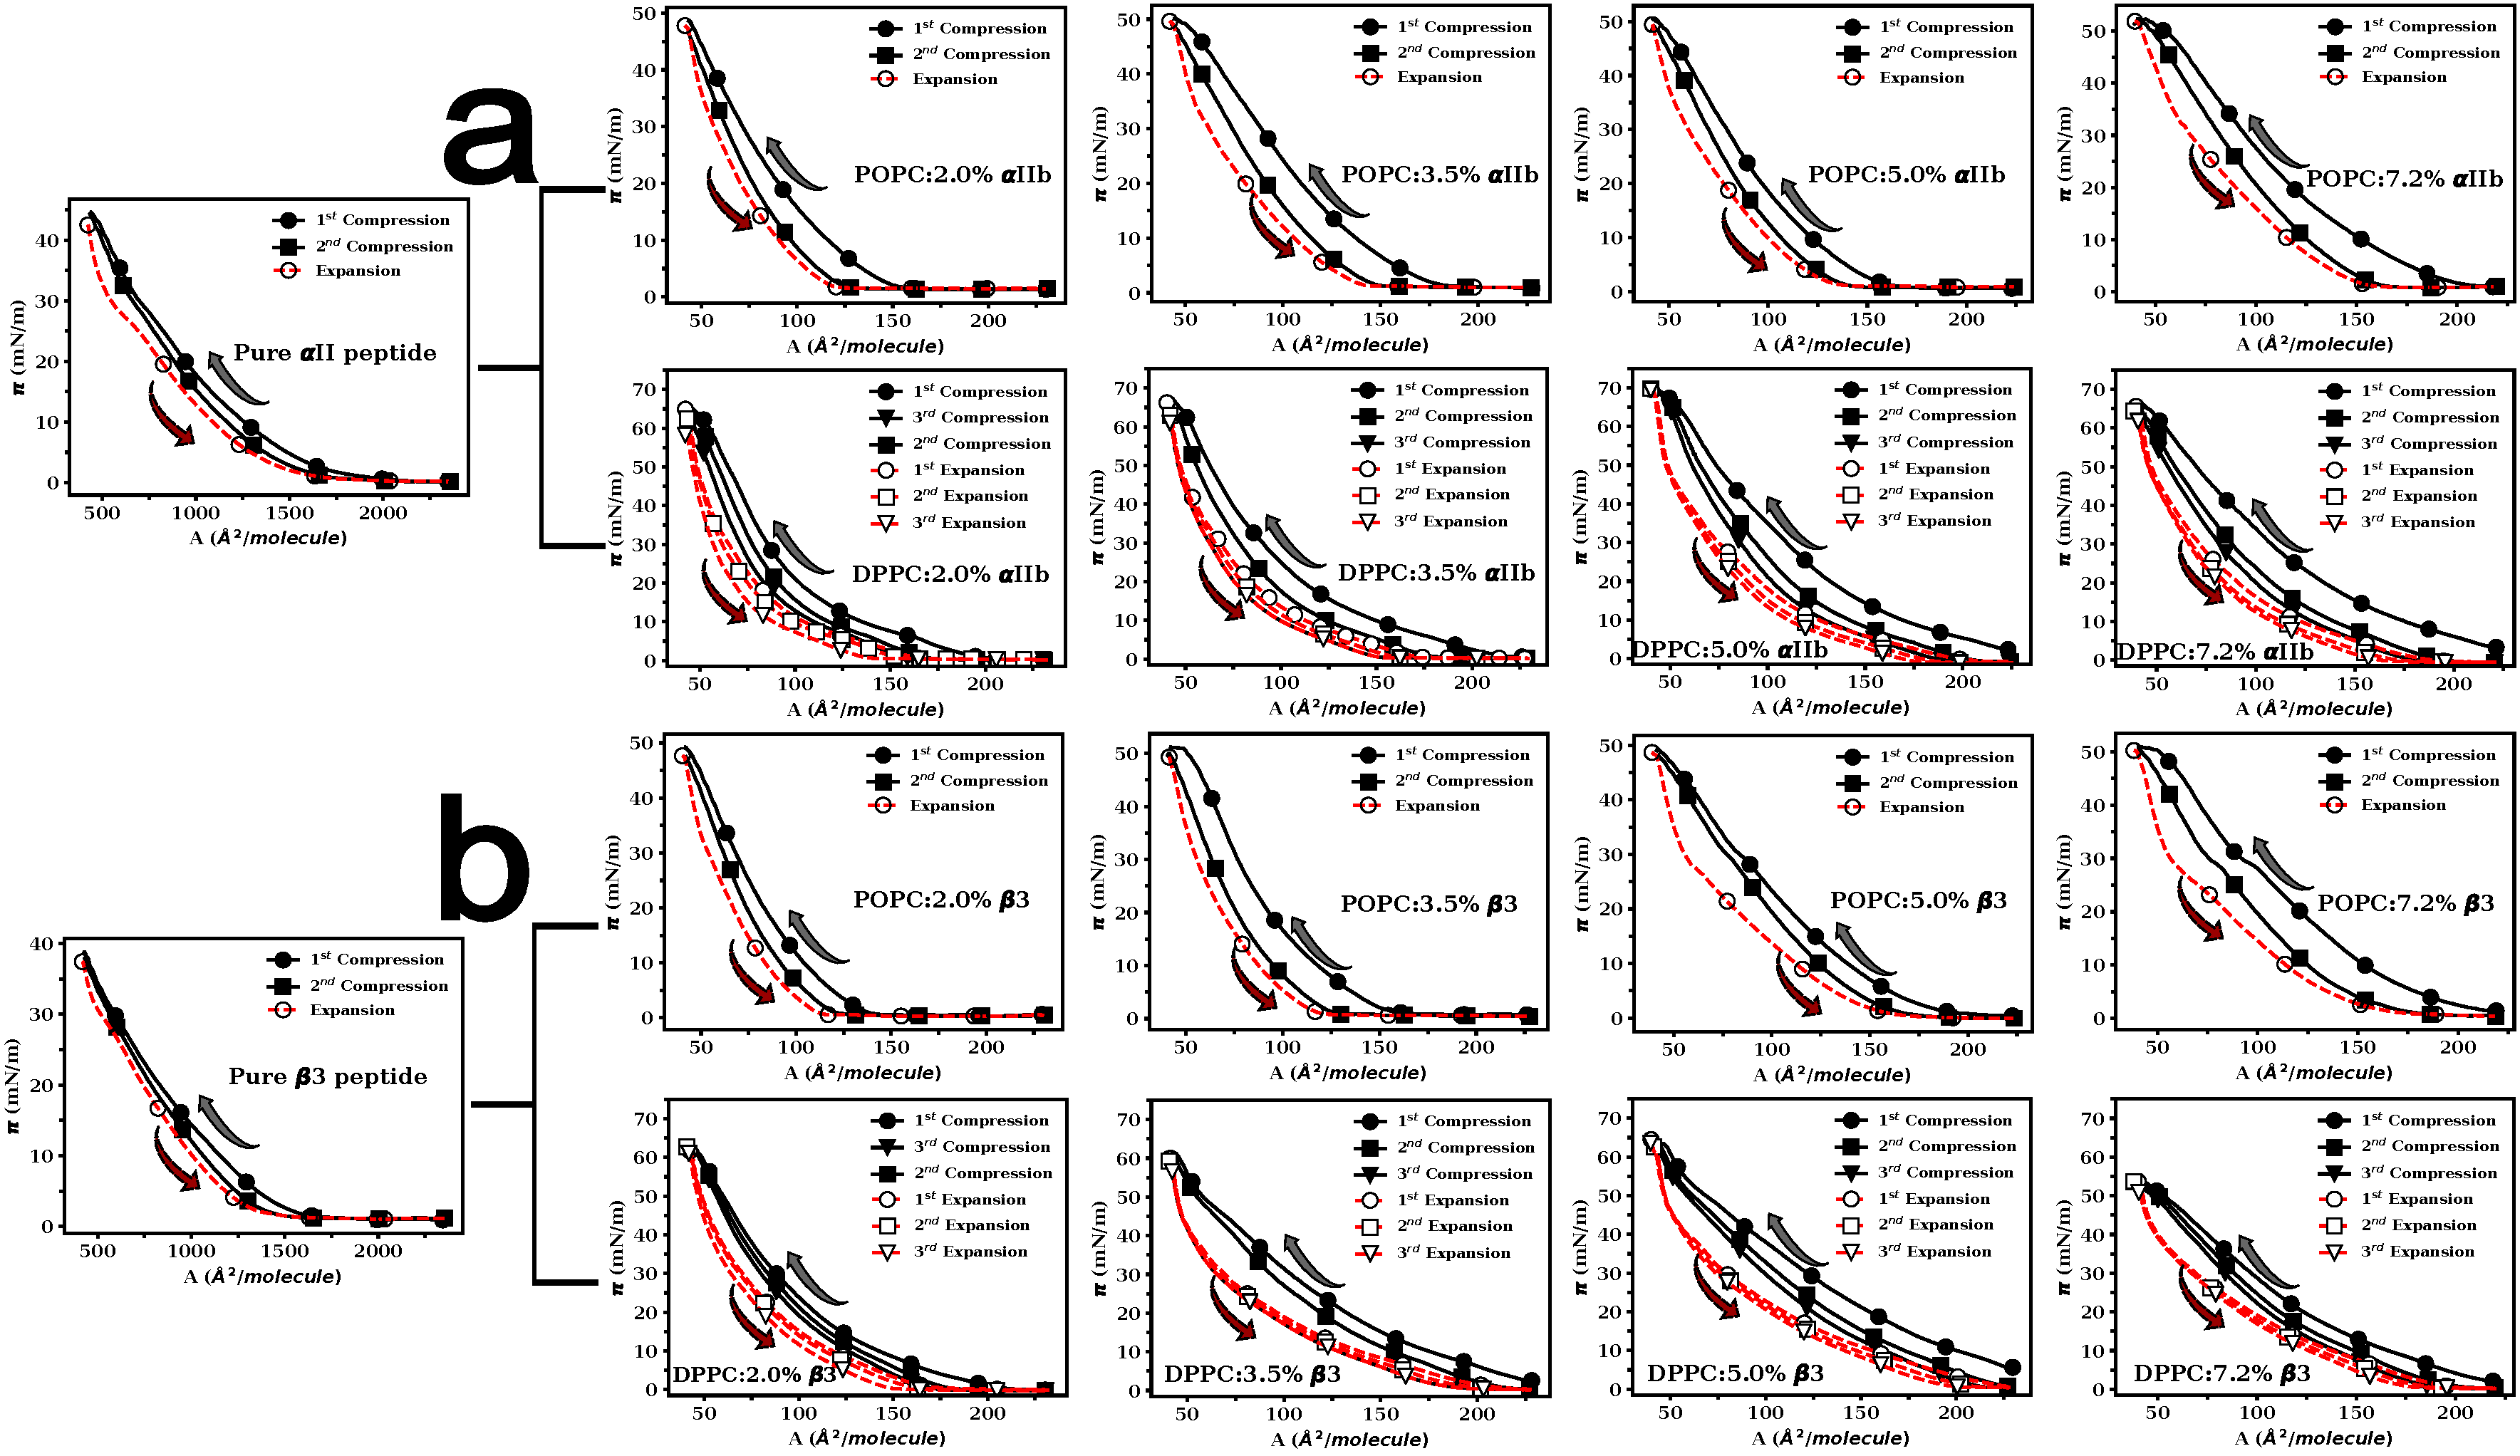
\includegraphics[width=1.0
    \linewidth]{fig/01_expe/mono/ciclos_comp_expa.pdf}
        \caption[compre-expan]{Histéresis de la compresión - expansión para las monocapas. \textbf{a-b)} POPC y \textbf{c-d)} DPPC}
        \index{compre_expan}
    \label{fig:compre_expan}
\end{figure}
\end{landscape}
%%%%%%%%%%%%%%%%%%%%%% Fin %%%%%%%%%%%%%%%%%%%%%%%%
%
